\chapter*{ВВЕДЕНИЕ}
\addcontentsline{toc}{chapter}{ВВЕДЕНИЕ}

Целью данного лаборотоной работы является проектирование и разработка программную реализацию машины "Энигмы".

Чтобы достигнуть поставленной цели, требуется решить следующие задачи:
\begin{itemize}
	\item провести анализ работы шифровальной машины "Энигмы";
	\item описать алгоритм шифрования;
	\item реализовать алгоритм шифрования.  
\end{itemize}

\chapter{Аналитическая часть}

\section{Определения}

\textbf{Информация}  --- сведения (сообщения, данные) независимо от формы их представления (накопленный опыт человечества).

\textbf{Защита информации} --- принятие мер
\begin{itemize}[label=---]
    \item нормативно-правовых (законы),
    \item организационно-структурных (внутренние правила организации, направленные на людей),
    \item технических (программные и аппаратные средства, физическая защита),
\end{itemize}
направленных на:
\begin{enumerate}
    \item предотвращение неправомерных действий в отношении информации:
    \begin{itemize}[label=---]
        \item доступ
        \item копирование
        \item модифицирование (изменение)
        \item блокирование
        \item предоставление (определенный круг лиц)
        \item распространение (неопределенный круг лиц)
        \item уничтожение (удаление)
    \end{itemize}
    \item соблюдение конфиденциальности информации ограниченного доступа,
    \item реализацию права на доступ к информации.
\end{enumerate}

\textbf{Актив} ---  все, что имеет ценность для субъекта и находится в его распоряжении.

\textbf{Информационная сфера:}
\begin{itemize}
    \item информация,
    \item информационная инфраструктура (SW, HW, коммуникации),
    \item субъекты, обрабатывающих информацию,
    \item процедуры (что делаем),
    \item система регулирования отношений (что, где, кем, как) --- как управлять.
\end{itemize}

\textbf{Угроза} --- опасность, предполагающая возможность потерь (ущерба).

\textbf{Безопасность} --- состояние защищенности интересов (целей) в условиях угроз.

\textbf{Информационная безопасность} --- безопасность в условиях угроз в информационной сфере

\textbf{Шифровальная машина "Энигма"} --- переносная электромеханическая машина, в которой электрическая схема меняется для каждой следующей буквы (многоалфавитный алгоритм)


\textbf{Одноалфавитная подстановка} --- подстановка, при которой каждый символ открытого текста заменяется на некоторый, фиксированный при данном ключе символ того же алфавита. Все варианты одноалфавитной подстановки букв сводятся к замене по формуле:
C(s)=(А(s)+B) mod D, где А-множитель, В-сдвиг, D-длина алфавита.

\textbf{Многоалфавитные подстановки} --- маскируют естественную частотную статистику языка. Для каждой буквы алфавита строится массив символов замены такие, что:
\begin{enumerate}
    \item ни одна пара массивов не пересекается, т.е. не содержит одинаковых элементов.
    \item количество символов замены в каждом массиве пропорционально частоте появления буквы в открытом тексте.
\end{enumerate}
Скрывается частота появления символа.

\section{Алгоритм шифрования Энигмы}

\textbf{Шифровальная машина "Энигма"} --- переносная электромеханическая машина, в которой электрическая схема меняется для каждой следующей буквы (многоалфавитный алгоритм).

Шифровальная машина «Энигма» внешне выглядит как печатающая машинка, за исключением того факта, что шифруемые символы не печатаются автоматически на определённый лист бумаги, а указываются на панели посредством загорания лампочки.

Шифровальная машина «Энигма» обладает тремя основными механизмами.
\begin{enumerate}
	\item Роторы --- cердце всех шифровальных машин, которое со стороны классической криптографии они реализуют полиалфавитный алгоритм шифрования, а их определённо выстроенная позиция представляет собой один из основных ключей шифрования. 
	Каждый ротор не эквивалентен другому ротору, потому как обладает своей специфичной настройкой. Военным на выбор давалось пять роторов, три из которых они вставляли в «Энигму».
	\item Рефлектор --- cтатичный механизм, позволяющий шифровальным машинам типа «Энигма» не вводить помимо операции шифрования дополнительную операцию расшифрования. Связано это с тем, что в терминологии классической криптографии рефлектор представляет собой просто частный случай моноалфавитного шифра.
	\item Коммутатор --- механизм, позволяющий оператору шифровальной машины варьировать содержимое проводов, попарно соединяющих буквы английского алфавита.
\end{enumerate}

Перед расшифровкой роторы возвращаются в начальное состояние. Расшифровка идентична шифрованию.

На рисунке~\ref{fig:enigma_example} представлена визуализация работы шифровальной машины "Энигма" на алфавите из восьми символов --- $\{A, B, C, D, E, F, G, H\}$.

\begin{figure}[h]
    \centering
    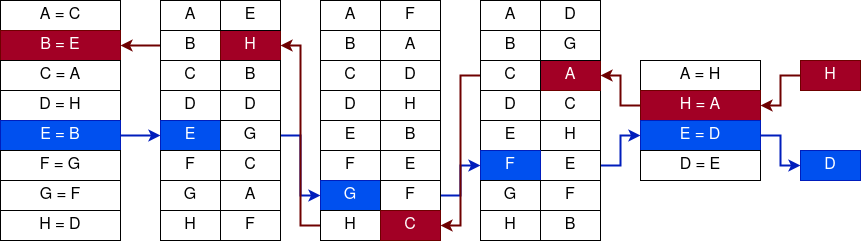
\includegraphics[width=1\linewidth]{images/example.png}
    \caption{Пример работы шифровальной машины "Энигма"}
    \label{fig:enigma_example}
\end{figure}



\chapter{Конструкторская часть}

\section{Схема алгоритма}

Схема алгоритма Энигмы представлена на рисунке~\ref{fig:enigma}.

\begin{figure}[h]
    \centering
    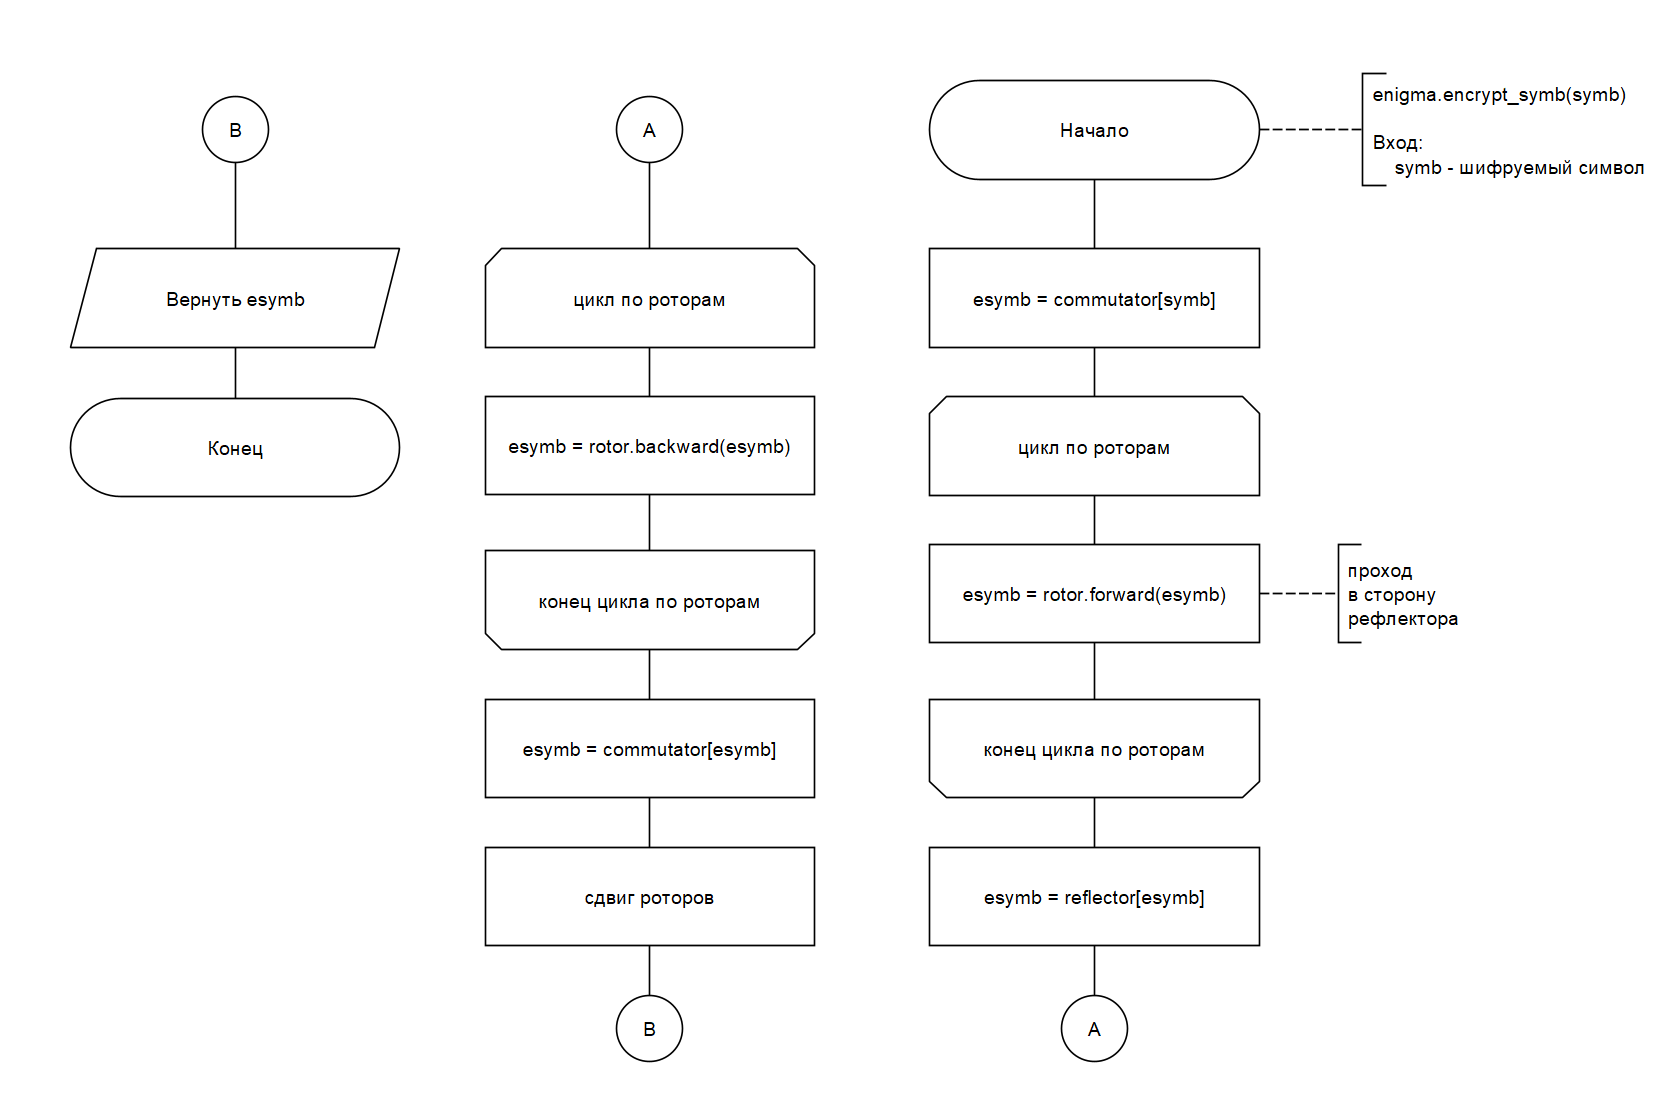
\includegraphics[width=1\linewidth]{images/sheme.png}
    \caption{Схема алгоритма шифровальной машины "Энигма"}
    \label{fig:enigma}
\end{figure}

